\documentclass[12pt]{article}


\usepackage{amssymb}
\usepackage{amsmath}
\usepackage{fullpage}
\usepackage{epsfig}
\usepackage{epstopdf}
\everymath{\displaystyle}
\usepackage{enumerate}

\newif\ifans

\anstrue

\begin{document}

\begin{center}
\underline{\LARGE{Chapter 4.1: Natural Logarithm \& The Number $e$}}
\end{center}

\subsection*{Expected Skills:}

\begin{itemize}

\item Be able to specify the domain and range of $f(x)=e^x$ and $f(x)=\ln{x}$.

\item Be able to graph $f(x)=e^x$ and $f(x)=\ln{x}$, labeling all intersections with the coordinate axes and all asymptotes.

\item Be able to solve equations involving the natural logarithm or exponential function.

\item Be able to evaluate limits involving the exponential function of the natural log function.

\item Be able to differentiate the exponential function or the natural log function; also, be able to solve application problems such as tangent line, rates of change, local/absolute extrema, and curve sketching.

\item Be able to perform logarithmic differentiation.

\end{itemize}

\subsection*{Practice Problems: }

%%%%%%%%%%
\subsubsection*{Algebraic Questions}

\begin{enumerate}

\item Approximate each of the following quantities using 3 rectangles of equal width and left endpoints, as described in the lecture notes.  Determine whether your approximation is an over approximation or an under approximation.

\begin{enumerate}

\item $\ln{4}$

\ifans\fbox{1.833333333; over approximation}\fi

\item $\ln{6}$

\ifans\fbox{2.676282051; over approximation}\fi

\end{enumerate}

\item Approximate each of the following quantities using 3 rectangles of equal width and right endpoints, as described in the lecture notes.   Determine whether your approximation is an over approximation or an under approximation.

\begin{enumerate}

\item $\ln{4}$

\ifans{\fbox{1.083333333; under approximation}}\fi

\item $\ln{6}$

\ifans{\fbox{1.287393162; under approximation}}\fi

\end{enumerate}

\newpage

\item Evaluate each of the following without using a calculator.

\begin{enumerate}

\item $\ln{1}$

\ifans\fbox{0}\fi

\item $\ln{e}$

\ifans\fbox{1}\fi

\item $\ln(e^2)$

\ifans\fbox{2}\fi

\item $\ln{\sqrt[3]{e}}$

\ifans\fbox{$\frac{1}{3}$} \fi

\item $e^{\ln{7}}$

\ifans\fbox{7}\fi

\item $e^0$

\ifans\fbox{1}\fi

\end{enumerate}

\item Use the properties of logarithms to expand (as much as possible) the expression as a sum, difference, and/or constant multiple of logarithms.  (Assume that all variables are positive.)

\begin{enumerate}

\item $\displaystyle \ln{(5x^{2}\sqrt{y})}$

\ifans\fbox{$\displaystyle \ln{5}+2\ln{x}+\frac{1}{2}\ln{y}$} \fi

\item $\displaystyle \ln{\frac{x^3}{y^2z^4}}$

\ifans\fbox{$\displaystyle 3\ln{x}-2\ln{y}-4\ln{z}$} \fi

\item $\displaystyle \ln{\sqrt[4]{x^{3}(x^{2}+3)}}$

\ifans\fbox{$\displaystyle \frac{3}{4}\ln{x}+\frac{1}{4}\ln{(x^{2}+3)}$} \fi

\end{enumerate}

\item Use the properties of logarithms to condense the expression to the logarithm of a single quantity.

\begin{enumerate}

\item $\displaystyle \ln{2}+\ln{x}$

\ifans\fbox{$\ln{(2x)}$} \fi
 
\item $\displaystyle 3\ln{x}+4\ln{y}-4\ln{z}$

\ifans\fbox{$\displaystyle \ln{\left(\frac{x^{3}y^{4}}{z^{4}}\right)}$} \fi

\end{enumerate}

\item Solve the given equation for $x$.  Where appropriate, you may leave your answers in logarithmic form.

\begin{enumerate}

\item $\displaystyle e^{x}+5=60$

\ifans\fbox{$x=\ln{55}$} \fi

\item $\displaystyle 11e^{x}+5=60$

\ifans\fbox{$x=\ln{5}$} \fi

\item $\displaystyle \left(3^{x-5}\right)-4=11$

\ifans\fbox{$\displaystyle x=\frac{\ln{15}}{\ln{3}}+5$} \fi

\item $\displaystyle \ln{x}-\ln{(x+1)}=2$

\ifans\fbox{No Solution} \fi

\item $\displaystyle \frac{1+\ln{x}}{2}=0$

\ifans\fbox{$\displaystyle x=e^{-1}$} \fi

\end{enumerate}

\item The equation $Q(t)=30e^{-4t}$ gives the mass (in grams) of a radioactive element that will {\bf remain} from some initial quantity after $t$ hours of radioactive decay.

\begin{enumerate}

\item How many grams were there initially?

\ifans\fbox{30 grams} \fi

\item  How long will it take for 40\% of the element to {\bf decay}?  You may leave your answer in logarithmic form.

\ifans\fbox{$\displaystyle -\frac{1}{4}\ln{\frac{3}{5}}$ hours} \fi

\end{enumerate}

\item In a research experiment the population of a certain species is given by $P(t)=15(7^t)$, where $t$ is the number of weeks since the beginning of the experiment.

\begin{enumerate}

\item How large was the population at the beginning of the experiment?

\ifans\fbox{15} \fi

\item How long will it take for the population to reach 300?  You may leave your answer in logarithmic form.

\ifans\fbox{$\displaystyle \frac{\ln{20}}{\ln{7}}$ weeks} \fi

\end{enumerate}

\end{enumerate}

%%%%%%%%%%
\subsubsection*{Limit \& Continuity Questions}

\noindent {\bf For problems 9-18, evaluate the following limits by first making an appropriate substitution.  If the limit does not exist, write DNE, $+\infty$, or $-\infty$ (whichever is most appropriate).}

\begin{enumerate}
\setcounter{enumi}{8}

\item  $\displaystyle \lim_{x\rightarrow \infty}{e^{x}}$ 

\ifans{\fbox{$+\infty$}} \fi

\item  $\displaystyle \lim_{x\rightarrow -\infty}{e^x}$ 

\ifans{\fbox{0}} \fi

\item  $\displaystyle \lim_{x\rightarrow -\infty}{\left(\frac{1}{e^x}\right)}$ 

\ifans{\fbox{$+\infty$}} \fi

\item  $\displaystyle \lim_{x\rightarrow \infty} e^{1/x}$ 

\ifans{\fbox{1}} \fi

\item $\displaystyle \lim_{x \rightarrow \infty}{\left(\frac{7}{e^x-8}\right)}$

\ifans{\fbox{0}} \fi

\item $\displaystyle \lim_{x \rightarrow -\infty}{\left(\frac{7}{e^x-8}\right)}$

\ifans{\fbox{$\displaystyle -\frac{7}{8}$}} \fi

\item $\displaystyle \lim_{x\rightarrow 0^+}{\ln{x}}$ 

\ifans{\fbox{$-\infty$}} \fi

\item  $\displaystyle \lim_{x\rightarrow \infty}{\ln{x}}$ 

\ifans{\fbox{$+\infty$}} \fi

\item $\displaystyle \lim_{x\rightarrow \infty}{\left(\frac{\ln{6x}}{\ln{2x}}\right)}$

\ifans{\fbox{1}} \fi

\item $\displaystyle \lim_{x\rightarrow \infty}{\left[\ln{(x+2)}-\ln{(3x+5)}\right]}$

\ifans{\fbox{$\displaystyle \ln{\left(\frac{1}{3}\right)}$}} \fi

\end{enumerate}

\noindent {\bf For problems 19-22, evaluate the following limits by first making an appropriate substitution.  If the limit does not exist, write DNE, $+\infty$, or $-\infty$ (whichever is most appropriate).}

\begin{enumerate}
\setcounter{enumi}{18}

\item $\displaystyle \lim_{x\rightarrow \infty}{\left(e^x \sin {(e^{-x})}\right)}$\\

\ifans{\fbox{1}} \fi

\item $\displaystyle \lim_{x\rightarrow 1}{\left(\frac{\sin{(\ln x^5)}}{\ln x}\right)}$ 

\ifans{\fbox{5}} \fi

\item $\displaystyle \lim_{x \rightarrow \frac{\pi}{2}^+}{e^{\sec{x}}}$

\ifans{\fbox{0}} \fi

\item $\displaystyle \lim_{x \rightarrow 0^+}{\tan^{-1}{(\ln{x})}}$

\ifans{\fbox{$\displaystyle -\frac{\pi}{2}$}} \fi

\end{enumerate}

%%%%%%%%%%
\subsubsection*{Derivative of the Natural Logarithmic Function}

\noindent {\bf For problems 23-35, calculate $\frac{dy}{dx}$.}

\begin{enumerate}
\setcounter{enumi}{22}

\item $y = \ln{(x^2)}$ 

\ifans{\fbox{$\frac{2}{x}$}} \fi

\item $y = \frac{1}{\ln{(3x)}}$ 

\ifans{\fbox{$-\frac{1}{x[\ln{(3x)}]^2}$}} \fi

\item $y = x^2\ln{x}$ 

\ifans{\fbox{$x+2x\ln{x}$}} \fi

\item $y = \ln{\left(\frac{1}{x}\right)}$ 

\ifans{\fbox{$-\frac{1}{x}$}} \fi

\item $y = \ln{(x^2+1)^2}$ 

\ifans{\fbox{$\frac{4x}{x^2+1}$}} \fi

\item $y = \left[\ln{(x^2+1)}\right]^2$ 

\ifans{\fbox{$\frac{4x\ln{(x^2+1)}}{x^2+1}$}} \fi

\item $y = \sqrt{\ln{2x}}$ 

\ifans{\fbox{$\frac{1}{2x\sqrt{\ln{(2x)}}}$}} \fi

\item $y = \tan{(\ln{x})}$ 

\ifans{\fbox{$\frac{1}{x}\sec^{2}(\ln{x})$}} \fi

\item $y = \ln{(\ln x)}$ 

\ifans{\fbox{$\frac{1}{x\ln{x}}$}} \fi

\item $y=\ln{|\sec{x}|}$

\ifans{\fbox{$\tan{x}$}} \fi

\item $y=\ln{|\sec{x}+\tan{x}|}$

\ifans{\fbox{$\sec{x}$}} \fi

\item $y=\ln{\left(x^x\right)}$

\ifans{\fbox{$1+\ln(x)$}} \fi

\item $y=\ln{\left(\frac{2x+1}{\sqrt{x}(3x-4)^{10}}\right)}$

\ifans{\fbox{$\frac{2}{2x+1}-\frac{1}{2x}-\frac{30}{3x-4}$}} \fi

\item Use logarithmic differentiation to calculate $\frac{dy}{dx}$ if $y=\frac{2x+1}{\sqrt{x}(3x-4)^{10}}$

\ifans{\fbox{$\frac{2x+1}{\sqrt{x}(3x-4)^{10}}\left(\frac{2}{2x+1}-\frac{1}{2x}-\frac{30}{3x-4}\right)$}} \fi

\item Let $y=x^{x^2}$.  Use logarithmic differentiation to calculate $\frac{dy}{dx}$.

\ifans{\fbox{$x^{x^2}(x+2x\ln{x})$}} \fi

\item Let $y=x^{\cos{x}}$.  Use logarithmic differentiation to calculate $\frac{dy}{dx}$.

\ifans{\fbox{$x^{\cos{x}}\left(\frac{\cos{x}}{x}-\sin{x}\ln{x}\right)$}} \fi


\item Compute an equation of the line which is tangent to the graph of $f(x)=\ln{(x^2-3)}$ at the point where $x=2$.

\ifans{\fbox{$y=4x-8$}} \fi

\item Find the value(s) of $x$ at which the tangent line to the graph of $y=\ln{(x^2+11)}$  is perpendicular to $y=-6x+5$.

\ifans{\fbox{$x=1$ and $x=11$}} \fi

\item Find the value(s) of $x$ at which the tangent line to the graph of $y=-\ln{x}$ passes through the origin.

\ifans{\fbox{$x=e$}} \fi

\item Calculate $\frac{d^2y}{dx^2}$ if $y=\ln{(3x^2+2)}$.

\ifans{\fbox{$\frac{12-18x^2}{(3x^2+2)^2}$}} \fi

\item Sketch $f(x)=\frac{\ln{x}}{x}$.  Label  the coordinates of all critical points, inflection points, $x$-intercepts, $y$-intercepts, and holes.  Also label all horizontal asymptotes and vertical asymptotes.

\ifans\fbox{\parbox{1\linewidth}{\begin{center}
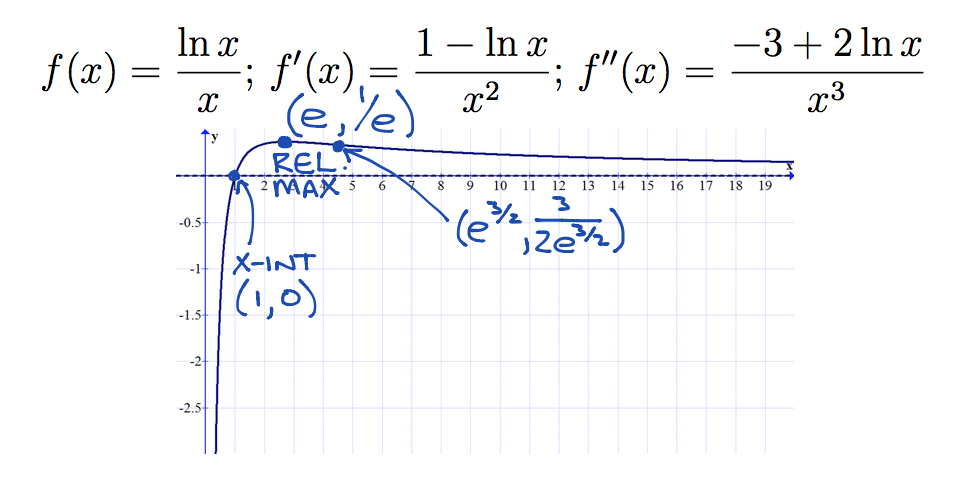
\includegraphics[scale=0.6]{9.png}
\end{center}
}}\fi


\item {\bf Multiple Choice:} Let $y=\ln{(\cos{x})}$.  Which of the following is $\frac{dy}{dx}$?

\begin{enumerate}

\item $(\ln{x})(-\sin{x})+(\cos{x})(\ln{x})$

\item $-\tan{x}$

\item $\cot{x}$

\item $\sec{x}$

\item $\frac{1}{\ln{(\cos{x})}}$

\end{enumerate}

\ifans{\fbox{B}} \fi

\item {\bf Multiple Choice:} Let $h(x)=\ln[(f(x))^2+1]$.  Suppose that $f(1)=-1$ and $f^{\prime}(1)=1$.  Find $h^{\prime}(1)$.

\begin{enumerate}

\item $-2$

\item $-1$

\item $0$

\item $1$

\item $2$

\end{enumerate}

\ifans{\fbox{B}} \fi

\item Consider the triangle formed by the tangent line to the graph of $y=-\ln{x}$ at the point $P(t,-\ln{t})$, the horizontal line which passes through $P$, and the $y$-axis. Find a function $A(t)$ which gives the area of this triangle.  

\ifans{\fbox{$A(t)=\frac{1}{2}t$}} \fi

\end{enumerate}

%%%%%%%%%%
\subsubsection*{Derivative of the Exponential Function}

\noindent{\bf For problems 47-57, differentiate.}

\begin{enumerate}
\setcounter{enumi}{46}

\item $y = e^{6x}$ 

\ifans{\fbox{$6e^{6x}$}} \fi

\item $g(x) = xe^{2x}$ 

\ifans{\fbox{$e^{2x}+2xe^{2x}$}} \fi

\item $y = e^x\cos {x}$ 

\ifans{\fbox{$-e^{x}\sin{x}+e^{x}\cos{x}$}} \fi

\item $g(x) = e^{x^2(x-1)}$ 

\ifans{\fbox{$e^{x^2(x-1)}(3x^2-2x)$}} \fi

\item $f(x) = \frac{1-e^{2x}}{1-e^x}$ 

\ifans{\fbox{$e^x$}} \fi

\item $f(x) = \frac{\ln{x}}{e^{x}+3x}$ 

\ifans{\fbox{$\frac{e^x+3x-x\ln{(x)}e^x-3x\ln{(x)}}{x(e^x+3x)^2}$}} \fi

\item $f(x) = \ln{(e^{x}+5)}$ 

\ifans{\fbox{$\frac{e^{x}}{e^{x}+5}$}} \fi

\item $f(x) = e^{\cos^2{2x}+\sin^2{2x}}$ 

\ifans{\fbox{0}} \fi

\item $h(x) = \exp{\left(\frac{1}{1-\ln x}\right)}$ 

\ifans{\fbox{$\frac{1}{x(1-\ln{x})^2}\exp{\left(\frac{1}{1-\ln x}\right)}$}} \fi

\item $f(x) = (\ln{x})^{e^{x}}$ 

\ifans{\fbox{$(\ln{x})^{e^{x}}\left(\frac{e^{x}}{x\ln{x}}+e^{x}\ln{(\ln{x})}\right)$}} \fi

\item $y = \frac{\arctan{(e^x)}}{x^3}$ 

\ifans{\fbox{$\frac{xe^{x}-3\tan^{-1}{(e^x)}-3e^{2x}\tan^{-1}{(e^x)}}{x^4(1+e^{2x})}$}} \fi

\item Compute an equation of the line which is tangent to the graph of $y=e^{3x}$ at the point where $x=\ln2$.

\ifans{\fbox{$y-8=24(x-\ln{2})$}} \fi

\item Compute an equation of the line which is tangent to the curve $e^{xy^2}+y=x^4$ at $(-1,0)$.

\ifans{\fbox{$y=-4x-4$}} \fi


\item Find a linear function $T_1(x)=mx+b$ which satisfies both of the following conditions:

\begin{itemize}

\item $T_1(x)$ has the same $y$-intercept as $f(x)=e^{2x}$.

\item $T_1(x)$ has the same slope as $f(x)=e^{2x}$ at the $y$-intercept.

\end{itemize}

\ifans{\fbox{$y=2x+1$}} \fi

\item The equation $y^{\prime \prime}+5y^{\prime}-6y=0$ is called a \underline{differential equation} because it involves an unknown function $y$ and its derivatives.  Find the value(s) of the constant $A$ for which $y=e^{Ax}$ satisfies this equation. 

\ifans{\fbox{$A=-6$ and $A=1$}} \fi

\item Sketch the given functions.  Label  the coordinates of all critical points, inflection points, $x$-intercepts, $y$-intercepts, and holes.  Also label all horizontal asymptotes and vertical asymptotes.

\begin{enumerate}

\item $f(x)=xe^{2x}$

\ifans\fbox{\parbox{1\linewidth}{\begin{center}
$f(x)=xe^{2x}$; $f^{\prime}(x)=e^{2x}(2x+1)$; $f^{\prime \prime}(x)=4e^{2x}(x+1)$\\
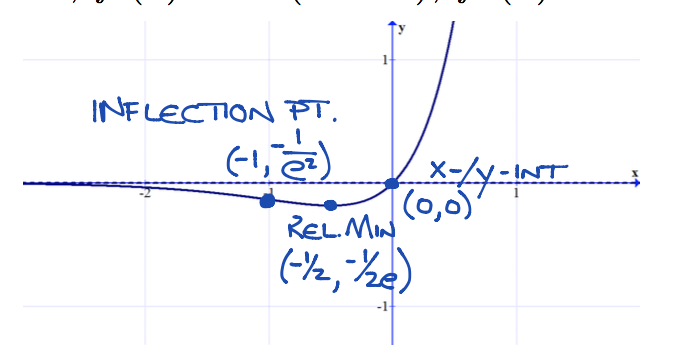
\includegraphics[scale=0.6]{7.png}
\end{center}
}}\fi

\item $f(x)=\frac{1}{\sqrt{2\pi}}e^{-x^2/2}$

\ifans\fbox{\parbox{1\linewidth}{\begin{center}
$f(x)=\frac{1}{\sqrt{2\pi}}e^{-x^2/2}$; $f^{\prime}(x)=-\frac{x}{\sqrt{2\pi}}e^{-x^2/2}$; $f^{\prime \prime}(x)=\frac{1}{\sqrt{2\pi}}e^{-x^2/2}(x^2-1)$\\
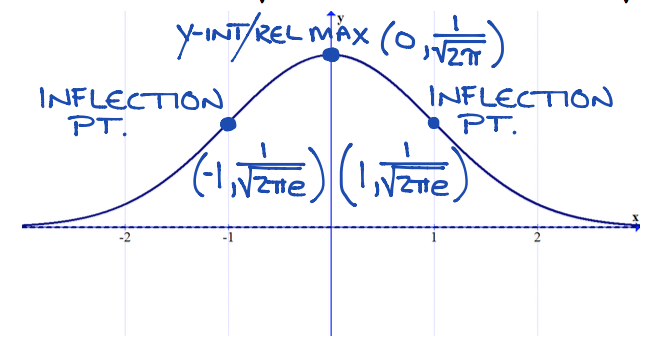
\includegraphics[scale=0.6]{8.png}
\end{center}
}}\fi

\end{enumerate}

\end{enumerate}

\end{document}